\documentclass[12pt, titlepage]{ctexrep}

\usepackage{amsmath}
\usepackage{amsfonts}

\usepackage[hidelinks]{hyperref}
\usepackage{fontspec}
% \usepackage{minted}
\usepackage{tikz}
\usepackage{float}
\usepackage{tikz-qtree}

\usetikzlibrary{arrows,shapes,positioning,shadows,trees}

\setmainfont{仿宋}
\setmonofont[Scale=.90]{DejaVu Sans Mono}
\author{武汉大学对不队}
\title{生物特征图像安全检索系统}

\linespread{1.5}

\pagestyle{headings}
\maketitle
\begin{document}

\tableofcontents


\chapter{摘要}
\label{chap:abstract}

信息技术的高速发展正在越来越快地将我们所居住的现实世界和我们所依赖的信
息世界整合起来,信息技术已经渗透进了我们生活中的点点滴滴。然而信息技术
的高速发展也带来了一些不小的威胁。在一般的内容检索系统中,应该被小心保
护起来的个人敏感数据并没有按照隐私保护的标准保存起来。

传统的内容检索系统仅着眼于访问控制以及数据传输的安全。虽然这两者能保证
数据可以安全到达服务端,但不能保证数据到达服务端后不被不法人员泄露。如
果单纯的使用加密算法来加密数据,服务端又不能利用传统的检索算法来按用户
的要求来搜索内容。

随着隐私信息数量的急剧增加和人们保护隐私意识的日益提高,研发在不牺牲数
据可用性和数据访问性的前提下、能更好地保护个人敏感信息的检索手段的需求
正在变得越来越大。

本系统从JPEG文件的压缩原理入手,利用Python以及一系列的开源函数库(
如numpy,opencv等),较好地实现了一个基于Logistic混沌系统的置乱加密算法
和基于离散余弦变换的内容检索系统。

该系统可以对固定大小的JPEG图像文件的加密,并在加密后保证了密图与原图的
统计特性相近,从而使得服务端可以对密图进行内容检索。并且加密速度与检索
速度较快。




\chapter{作品介绍}
\label{chap:intro}

\section{背景分析}
\label{sec:bkg-analysis}

信息技术的高速发展正在越来越快地将我们所居住的现实世界和我们所依赖的信
息世界整合起来。信息技术已经渗透进了我们生活中的点点滴滴:从使用搜索引
擎来检索信息,到在社交网络上分享用户产生内容(User Generated Content),
从个人信息管理(如电子邮件和在线相册),到网络备份服务,云计算时代已
经到来。

基于内容的图像检索系统(Content-based Image Retrieval System)也随着信
息科学技术的进步被发展出来被运用在云计算中,特别地、基于内容的生物特征
图像检索系统(Content-based Biometric Image Retrieval System)对生物特
征图像本身包含的视觉特征和语义信息等进行分析,提取其中能够有效表征图像
的重要特征,并对这些特征进行相似性比较,找出与待检索图像“相似”的生物特
征图像。由于这种基于图像特征的检索方法可以实现图像之间的量化分析与比较、
具有比较强的客观性、能快速有效地进行大量数据的分析与搜索,是一类应用非
常广泛的内容检索系统。

然而信息技术的高速发展也带来了一些不小的威胁。云计算如同一把双刃剑,社
会因云计算的普及而获益匪浅,但个人隐私也无处遁形。其因网络而泄露的事件
时有发生:如2011年3月谷歌邮箱的用户数据泄露事件、2011年4月索
尼PlayStation网络中7700万个注册账户持有人的个人信息失窃和2013年3月云计
算笔记应用Evernote泄露大量用户名、电子邮件地址与加密密码泄露事件等。这
些云计算安全事故给我们敲响了警钟,云安全的保障迫不及待。

在一般的生物特征内容检索系统中,不仅一般信息被存储起来以供后用,应该被
小心保护起来以防范未授权的访问的个人敏感数据(如指纹特征、人脸特征等),
也被按与一般信息同样的方法存储了起来。对于个人敏感信息的安全管理正在成
为一个越来越重要的问题。如果该问题能够得到一定程度的解决,内容检索系统
关于数据保密性和数据可用性的需求将得到一定程度的缓解。

传统的内容检索系统对于敏感信息的保护主要着眼于访问控制(Access Control)
以及安全的数据传输。这两者保证了数据可以安全地送达服务器,而且任何未授
权的人员都不能访问该数据。然而当数据到达服务器后,传统内容检索系统会解
密这些数据,并且直接对明文做归类、检索和数据分析。这就使得敏感信息可能
通过服务端被透露出去,例如敏感信息会对服务端玩忽职守的系统管理员或恶意
的入侵者以明文形式显示出来。

随着隐私信息数量的急剧增加、云计算安全事故的频发和人们保护隐私意识的日
益提高,研发在不牺牲数据可用性和数据可访问性的前提下、能更好地保护个人
敏感信息的检索手段的需求正变得越来越大。在这个趋势下,可以在加密的多媒
体数据库上实现基于内容检索的技术手段,会在帮助人们更快更安全地管理多媒
体数据和隐私中扮演越来越重要的角色。

\section{特色描述}
\label{sec:spec-description}

对服务端内数据的加密能够保护个人隐私信息免疫于服务端不受信任的访问。但
是如果仅使用传统加密算法,服务端将不能顺利处理数据,也就不能对用户的检
索请求产生结果。

基于加密数据库的内容检索,其目标是提供关于加密文档的、高效准确的搜索能
力,并且在搜索时应不需要先解密文档。即服务端仅提供存储和检索功能,不应
有解密个人敏感信息的能力,还应该保证服务端可以从用户数据集所获得的信息
量是最少的。

本系统从JPEG文件的压缩原理入手,实现了一个基于Logistic混沌系统的置乱加
解密算法和基于离散余弦变换的内容检索系统,并基于这两个算法,实现了一
个C/S构架的系统。其中客户端与服务端都由两部分(内核和前端)组成。

\subsection{系统方案特色}
\label{sec:sys-design-spec}
\begin{itemize}
\item 加密内容写回至JPEG文件,使加密内容可见,但不可理解。
\item 加密算法使用的是像素级置换,加解密速度较快。
\item 由于Logistics映射的优良性质\cite{li2011},加密算法的密钥空间至少高于128bit。
\item 禁止指纹相同的图片的多次存储,以防止数据库管理复制图片伪造身份。
\end{itemize}

\subsection{系统实现特色}
\label{sec:sys-impl-spec}
\begin{itemize}
\item 整个系统构建于经过广大用户验证过的开源库或开源程序上,可以保证软
件基础设施的安全性。
\item 系统构架为客户端/服务端,其中交互使用经过广泛使用的HTTP协议,使
一个服务器可以支持多个客户端同时访问,同时不增加服务端的程序复杂性。
\item 服务端使用简洁的Flask框架和支持高并发的tornado库,高效可靠。
\item 客户端使用了跨平台的Qt框架作为前端,内核算法使用了实现了多种快速
算法的OpenCV库和numpy库。
\item 客户端服务端的内核与前端分开,耦合度低,用户可以方便的进行二次开
发。
\end{itemize}

\section{相关工作}
\label{sec:related-work}
为了实现系统设计目标,我们研究了离散余弦变换和Logistic映射的性质及其应用。

\subsection{离散余弦变换}
离散余弦变换(以下简称DCT)是一种将时空域上的函数转换到频域的、具有良好能
量聚集性质的、存在快速算法的数学变换。其公式如下:
\begin{displaymath}
X_k = \frac1 2 \left[x_0 + \left(-1\right)^k x_{N - 1}\right] + \sum_{n = 1}^{N - 2} x_n \cos \left(
        \frac{\pi} {N - 1} n k \right) \qquad k = 0, \dotsc, N - 1
\end{displaymath}

JPEG图片格式利用了人眼对低频信号敏感、对高频信号不敏感的特点对高频信号
进行压缩。DCT使用最广泛的一种变形——二维DCT可以将良好的将高频与低频信
号分离。在JPEG编码中,整个图像数据(灰度值)按$8 \times 8$分块,每块经
过离散余弦变换、量化和熵编码之后按照JPEG标准编码到文件中。

二维DCT(DCT-II)公式如下:
\begin{displaymath}
X_k = \sum_{n = 0}^{N - 1} x_n \cos \left[\frac{\pi} N \left(n +
        \frac1 2\right) k\right] \qquad k = 0, \dotsc, N - 1
\end{displaymath}

在DCT-II中,输入矩阵$I$的能量被充分聚集到了左上角,其中输出矩阵$M$的
$M_{0, 0}$是最能代表输入矩阵的值,这个值被称为DC系数(直流系数),即输入
能量的均值。矩阵中其他的值被称为AC系数(交流系数)。
离DC系数越远的AC系数所代表的频率就越
高,人眼也就对它越不敏感。



\subsection{Logistic映射}
Logistic映射(或称单峰映射)是一种二次的多项式映射,是实际系统中存在的
最简单的非线性差分方程之一\cite{yang2011}。这个映射因生物学家Robert
May在1976年发表的一篇论文而著名。其公式如下:
\begin{displaymath}
x_{n + 1} = rx_n(1 - x_n) \qquad 0 < r \leq 4, r \in \mathbb{R}
\end{displaymath}

Logistic映射所构建的密钥序列具有良好的随机性和初值敏感性,当$r >
3.569945672\dotsb$时,系统进入混沌状态,产生的序列非周期不收敛,随着初
始值的不同有着非常大的差异性\cite{yang2011}。

混沌现象是在非线性动力系统中出现的、具有对初始条件的
敏感依赖性、类噪声、非周期性、确定性的、类随机的过程,这种过程既非周期
又不收敛,其状态完全可以重现\cite{lu2007}。故本系统选用该映射来生成混
沌序列,随后用该混沌序列来生成初始密钥敏感的伪随机序列,
最后利用多个伪随机序列构成置乱矩阵来加密输入图片。

\section{市场分析}
\label{sec:market-analysis}

基于加密数据库的信息检索是一项前景非常好的技术。在当今世界中,摄像头与
数码相机使用得越来越广泛,也就意味着数字多媒体信息的获取已经越来越容易,
而且正在快速渗透入多个方面,如医疗系统、刑侦系统等。

本系统实现了一个可以对固定规格的图像进行加密,并且能对密图进行检索的轻
量级系统。其对生物特征图像的检索效果突出,如人脸图、半身像等。其中加密
算法具有高速、密钥空间较大的特点,检索算法具有快速、简单的特点。可以在
具有大量相同模式的内容需要检索、且内容检索系统需要保证一定秘密性的领域
中使用,如医疗系统中的医疗图像内容检索系统等。由于可以实现拷贝检测,本
系统也可用于防止身份滥用的生物特征图像数据库中。


\chapter{系统设计}
\label{chap:sys-design}

\section{系统说明}
\label{sec:sys-description}
% Data flow diagram
% Author: David Fokkema
\pgfdeclarelayer{background}
\pgfdeclarelayer{foreground}
\pgfsetlayers{background,main,foreground}

\begin{figure}[H]

\caption{系统架构图示}
\label{fig:sys-arch}
\centering
\begin{tikzpicture}[
font=\sffamily,
    every matrix/.style={ampersand replacement=\&,column sep=1cm,row sep=1cm},
    source/.style={draw,thick,rounded corners,fill=red!20,inner sep=.3cm},
    process/.style={draw,thick,rounded corners,inner sep=.3cm,fill=blue!20},
    sink/.style={source,fill=green!20},
    to/.style={->,>=stealth',shorten >=1pt,semithick,font=\sffamily\footnotesize},
    every node/.style={align=center}]

    % Position the nodes using a matrix layout
    \matrix{
        \& \& \node[source] (inputimg) {录入图像}; \& \\
        \& \& \node[process] (correction) {矫正}; \& \\
        \node[source] (restoredimg) {还原图};
        \& \node (hiddennodeclient) {};
        \& \node[source] (ainputimg) {待添加图像};
        \& \node[source] (rinputimg) {待检索图像}; \\
          \node[process] (decimg) {解密 (逆置乱)};
        \& \& \node[process] (encimg) {加密 (置乱)};
        \& \node[process] (encimga) {加密 (置乱)}; \\
    \node (hiddenhttpa) {}; \& \node (hiddenhttpb) {};
      \& \node (hiddenhttpc) {}; \& \node (hiddenhttpd) {}; \\
    \node (hiddennodeserver) {};
       \& \& \node[process] (extfeat) {提取特征}; 
       \& \node[process] (extfeata) {提取特征}; \\
    \node[source] (results) {匹配结果};
        \& \node[sink] (imgdb) {图片数据库};
        \& \node[sink] (featdb) {特征数据库};
        \& \node (rightbottom) {}; \\
  };

  \path (hiddennodeclient.south) + (0, -0.5) node (client)
      {\Large \emph{客户端}};
  \path (hiddennodeserver.east) + (1.8, -0.2) node (server) {\Large
     \emph{服务端}};
  \path (hiddenhttpa.east) + (1.8, 0) node (http-level)
      {\Large \emph{HTTP}};

  % Draw the arrows between the nodes and label them.
  \draw[to] (decimg) -- (restoredimg);
  \draw[to] (results) -- (decimg);
  \draw[to] (inputimg) -- (correction);
  \draw[to] (correction) -- (ainputimg);
  \draw[to] (ainputimg) -- (encimg);
  \draw[to] (encimg) -| node[midway, above] {加入} (imgdb);
  \draw[to] (encimg) -- (extfeat);
  \draw[to] (extfeat) -- node[midway, left] {加入} (featdb);
  \draw[to] (rinputimg) -- (encimga);
  \draw[to] (encimga) -- (extfeata);
  \draw[to] (extfeata) |- node[midway, below] {比对} (featdb);
  \draw[to] (featdb) -- (imgdb);
  \draw[to] (imgdb) -- (results);

  \begin{pgfonlayer}{background}
    \path (decimg.west |- rinputimg.north) + (-0.3, 0.3) node
    (a) {};
    \path (encimg.south -| rinputimg.east) + (+0.3, -0.3) node (b)
    {};
    \path[fill=cyan!10, rounded corners, draw=black!50, dashed] (a)
    rectangle (b);
    \path (extfeat.north -| extfeata.east) + (+0.5, +0.3) node (a) {};
    \path (results.west |- imgdb.south) + (-0.7, -0.3) node (b) {};
    \path[fill=yellow!10, rounded corners, draw=black!50, dashed] (a)
    rectangle (b);
    \path (hiddenhttpa.west |- hiddenhttpd.north) + (-1.7, 0.3) node
    (a) {};
    \path (hiddenhttpc.south -| hiddenhttpd.east) + (+1.5, -0.3) node
    (b) {};
    \path[fill=gray!10, rounded corners, draw=black!50, dashed] (a)
    rectangle (b);
  \end{pgfonlayer}

\end{tikzpicture}


\end{figure}



\section{设计目标}
\label{sec:design-goal}

\section{系统架构}
\label{sec:sys-arch}

系统由客户端和服务端组成。

\subsection{客户端}
客户端由前端模块(\texttt{ui.py})和核心模块(\texttt{libs}包)构成,
而核心模块又由\texttt{ClientCore}类(\texttt{libs/core.py})和
\texttt{LogisticPermutation}类(\texttt{libs/logistic.py})组成。其中
\begin{itemize}
\item \texttt{ClientCore}类负责图像的加解密与服务器的交互(例如上传图
  片至数据库或请求检索图片等);
\item \texttt{LogisticPermutation}类负责根据给定的初始密钥求出加解密置
  换表。
\end{itemize}

\subsection{服务端}

\section{功能原理及实现}
\label{sec:func-impl}

为了达到标准化图片库,便于实现功能的目的,本系统只接受宽$640$像素,高
$480$像素,即$4:3$的灰度JPEG图片。

\subsection{检索匹配方面}
\label{sec:retrieval-impl}
本系统利用二维DCT抽取出一张图片的特征向量。具体方法如下:
\begin{enumerate}
\item 将输入JPEG图片按$8 \times 8$分块,对每块做DCT;
\item 取每块的DC系数,添加到数组$V$中;
\item 将$V$按降序排序,得到$W$,并取$W$的前$n$个元素作为该输入图片的特征向量。
\end{enumerate}

其中$n$可以根据实际需要来取。由于$W$中下标越大的元素,其值越小,在向量
距离计算中起到的作用就越小,因此本系统实现中对检索效果和效率进行衡量,
选择了$128$作为该参数的值。

计算距离方面使用的是numpy库中的\texttt{linalg.norm}函数。

\subsection{加解密方面}
\label{sec:enc-dec-impl}

本系统使用的加解密算法的初始密钥由三组$x_0$,$r$,$s$组成,
其中$x_0 \in (-1, 1)$,$r \in [3.57, 4]$,$s > 0, s \in \mathbb{Z}$。

加密算法首先使用伪随机序列生成算法生成若干置乱表,然后根据置乱表对图片
进行块内和块间的置乱达到使图片不可理解、但保留DC系数的统计特性的目的。
解密算法与加密算法类似,只是使用的置乱表不一样,即加解密算法是对合的。

由Logistic映射生成具有$n$个元素的伪随机序列的具体做法\cite{lu2007}是:
\begin{enumerate}
  \item 使用初始密钥$x_0$和$r$,迭代Logistic公式,生成具有$n + s$个元
      素的混沌序列,并舍去前$s$个元素,得到$L = \{x_1, x_2, x_3, \dotsc, x_n\}$;
  \item 对$L$进行升序排序,得到$M = \{x_1^\prime, x_2^\prime, x_3^\prime,
      \dotsc, x_n^\prime\}$;
  \item 定位$x_i$在$x_i^\prime$中的位置序数,得到序数序列,记为$P =
      \{p_1, p_2, p_3, \dotsc, p_n\}$
\end{enumerate}
$P$就是所求的关于初始密钥$x_0$、$r$和$s$的伪随机序列。

由置乱表生成逆置乱表的具体做法是:
\begin{enumerate}
  \item 扩展输入序列为$P^\prime = \{(0, x_1), (1, x_2), (2, x_3),
      \dotsc, (n - 1, x_n)\} & \quad x_i \in P$;
  \item 建立一个新表$I$,使得$\forall (i, x_{i + 1}) \in P^\prime$,
      $I_{x_{i + 1}} = i$
\end{enumerate}
$I$就是所求的关于$P$的逆置乱表。

本系统为了保证每个DCT块的均值不变,利用不同的初始密钥生成了3个伪随机序列,分别是:
\begin{itemize}
  \item 利用第一组初始密钥生成了具有$w$个元素的$T_{column}$,作为块间的列置乱表;
  \item 利用第二组初始密钥生成了具有$h$个元素的$T_{row}$,作为块间的行置乱表;
  \item 利用第三组初始密钥生成了具有64个元素的$T_{block}$,作为DCT块内的置乱表;
\end{itemize}
其中$w$等于图片宽度除以$8$,$h$等于图片宽度除以$8$。



\newcommand{\insimg}[1] {
  \begin{subfigure}[b]{0.2\textwidth}
    \centering
    \includegraphics[keepaspectratio=true, width=\textwidth]{images/#1}
  \end{subfigure}
}

\chapter{性能测试}
\label{chap:benchmark}

为了测试本系统的可用性,需要测试检索算法的鲁棒性和效率。

\section{测试指标}
\label{sec:benchmark-index}
鲁棒性:本系统利用DCT抽取出图像的特征向量,采用向量间的距离作为图片的
相似程度的度量,距离越大,图片相似程度越低,同理,距离越小(大于0),
图片的相似程度就越高。对鲁棒性的测试应着眼于在不同情况下,加噪图与
原图的距离的变化情况,距离越小,抗噪声性能越好。

效率:本系统接受一个待检索图后,在特征数据库中检索所有的特征向量后返回
前10相似的图片。对效率的测试应着眼于系统检索出结果的时间,以及客户端接
收到全部结果图片的时间,检索时间越小,服务端检索性能越好,接受时间越
小,客户端性能越好。

\section{测试方案}
\label{sec:benchmark-scheme}

\begin{itemize}
\item 为了测试检索算法的鲁棒性,拟选择一些样本图片,并对这些样本做一些典型的
变化:
\begin{itemize}
\item 加入椒盐噪声
\item 改变质量因子$Q$
\end{itemize}
然后统计加噪图与原图的距离。

\item 为了测试检索算法的效率,拟在同一台主机上同时开启本系统的服务端和客户端,
即在忽略网络状况的情况下测试系统的检索速度并统计时间。
\end{itemize}

\section{测试环境}
\label{sec:benchmark-env}

\begin{itemize}
\item 硬件环境:
\begin{itemize}
\item 处理器:Intel Core i5-2410M CPU @ 2.30GHz
\item 内存:4.00GB(3.82GB可用)
\end{itemize}
\item 软件环境:
\begin{itemize}
\item 操作系统:Windows 8 专业版 x64(含Media Center) 
\item Python 2.7.3 x86
\item numpy 1.7.1
\item opencv-python-2.4.5
\end{itemize}
\end{itemize}

\section{测试数据}
\label{sec:benchmark-data}

测试图像集为37张灰度人脸图,大小为$640 \times 480$,单位为像素。
图集如下图

\begin{figure}[H]
  \centering
  \insimg{gs0.jpg}
  \insimg{gs1.jpg}
  \insimg{gs2.jpg}
  \insimg{gs3.jpg}
  \vspace{0.1cm}

  \insimg{gs4.jpg}
  \insimg{gs5.jpg}
  \insimg{gs6.jpg}
  \insimg{gs7.jpg}
  \vspace{0.1cm}

  \insimg{gs8.jpg}
  \insimg{gs9.jpg}
  \insimg{gs10.jpg}
  \insimg{gs11.jpg}
  \vspace{0.1cm}

  \insimg{gs12.jpg}
  \insimg{gs13.jpg}
  \insimg{gs14.jpg}
  \insimg{gs15.jpg}
  \vspace{0.1cm}

  \insimg{gs16.jpg}
  \insimg{gs17.jpg}
  \insimg{gs18.jpg}
  \insimg{gs19.jpg}
  \vspace{0.1cm}
\end{figure}
\begin{figure}[H]
  \centering

  \insimg{gs20.jpg}
  \insimg{gs21.jpg}
  \insimg{gs22.jpg}
  \insimg{gs23.jpg}
  \vspace{0.1cm}

  \insimg{gs24.jpg}
  \insimg{gs25.jpg}
  \insimg{gs26.jpg}
  \insimg{gs27.jpg}
  \vspace{0.1cm}

  \insimg{gs28.jpg}
  \insimg{gs29.jpg}
  \insimg{gs30.jpg}
  \insimg{gs31.jpg}
  \vspace{0.1cm}

  \insimg{gs32.jpg}
  \insimg{gs33.jpg}
  \insimg{gs34.jpg}
  \insimg{gs35.jpg}
  \vspace{0.1cm}

  \insimg{gs36.jpg}
\end{figure}


\section{测试结果及分析}
\label{sec:result-and-analysis}

\subsection{椒盐噪声}
\label{sec:speckle-data}

典型的加入椒盐噪声的图如下
\begin{figure}[H]
  \centering
  \begin{subfigure}[b]{0.4\textwidth}
    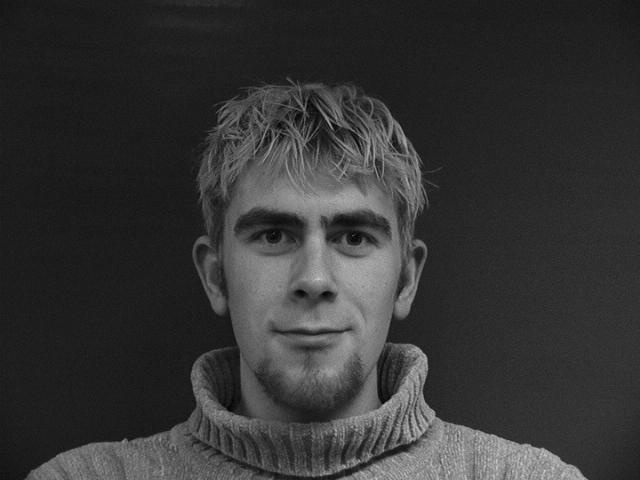
\includegraphics[keepaspectratio=true,
    width=\textwidth]{images/gs0.jpg}
    \caption{原图}
  \end{subfigure}
  \begin{subfigure}[b]{0.4\textwidth}
    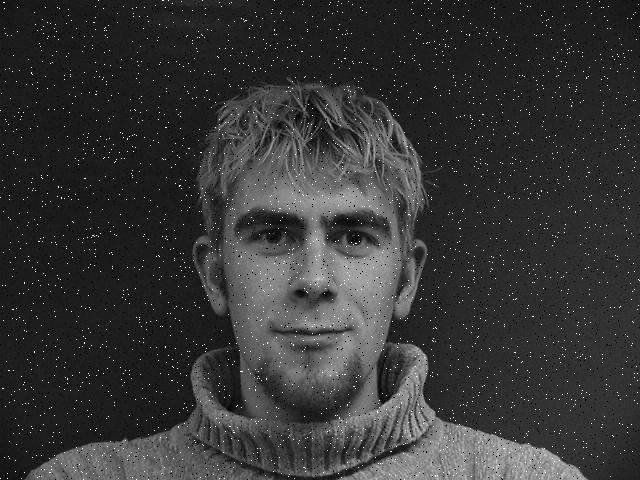
\includegraphics[keepaspectratio=true,
    width=\textwidth]{images/gs0_0.02_speckle.jpg}
    \caption{加噪图}
  \end{subfigure}
  \caption{噪声参数为0.02时的椒盐噪声对gs0.jpg的影响}
\label{fig:speckle-ex-img}
\end{figure}

对上示原图加入噪声密度在$[0, 0.1]$内、步长为0.01的椒盐噪声后,分别统计
与原图的距离,可作如下的散点图
\begin{figure}[H]
  \centering
  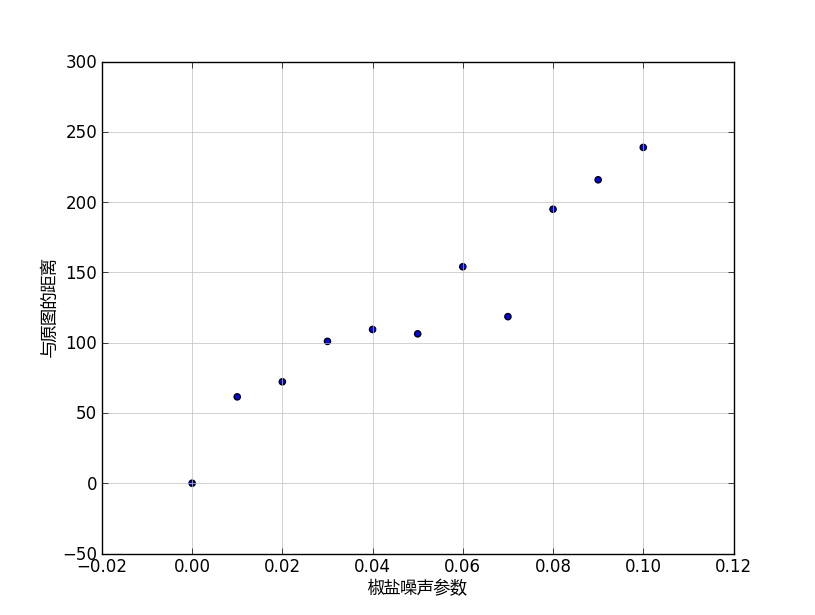
\includegraphics[keepaspectratio=true,
  scale=0.6]{images/speckle_gs0.png}
  \caption{对gs0.jpg的椒盐噪声统计}
  \label{fig:speckle-gs0-scatter-plot}
\end{figure}

为不失一般性,选取37张图片做同样处理,统计出散点图,如图
\begin{figure}[H]
  \centering
  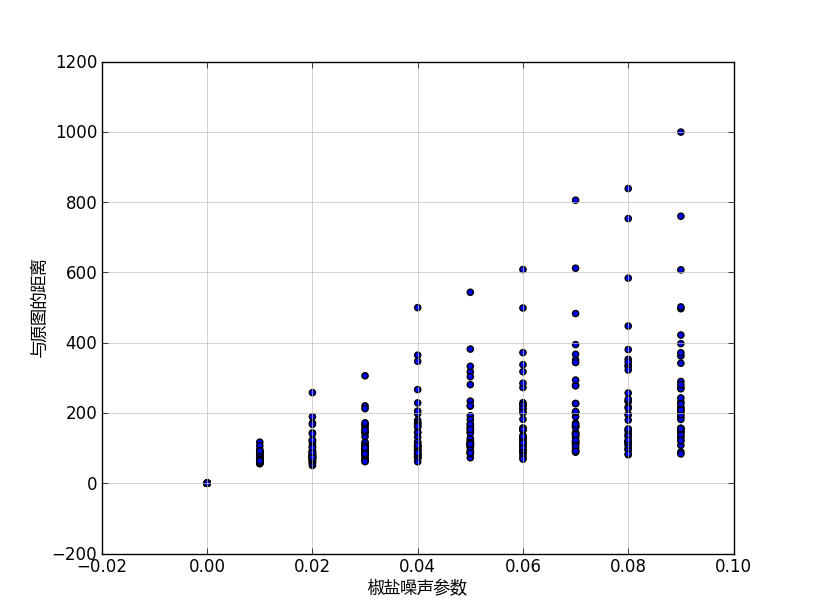
\includegraphics[keepaspectratio=true,
  scale=0.6]{images/speckle_all.png}
  \caption{对所有图片的椒盐噪声统计}
  \label{fig:speckle-all-scatter-plot}
\end{figure}

从图中可以看出来,本算法可以抵抗噪声密度小于$0.1$的椒盐噪声,在此噪声
密度下,加噪图与原图距离普遍小于$500$,当噪声密度大于$0.1$后,加噪图
与原图距离增大到了无法接受的地步。

\subsection{质量因子}
\label{sec:quality-data}

原图与质量因子$Q = 10$时的图如下
\begin{figure}[H]
  \centering
  \begin{subfigure}[b]{0.4\textwidth}
    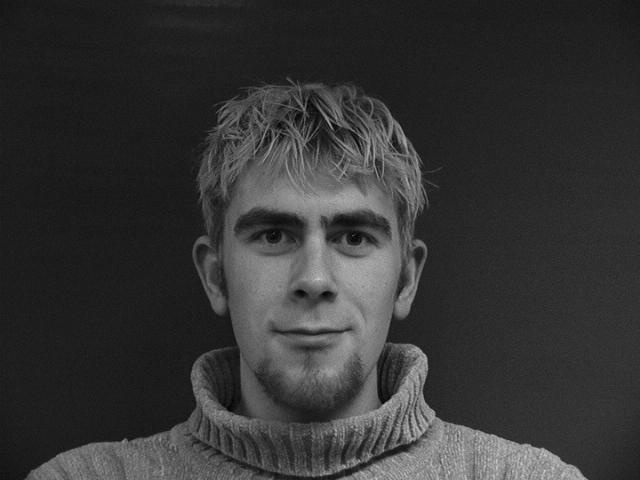
\includegraphics[keepaspectratio=true,
    width=\textwidth]{images/gs0.jpg}
    \caption{原图}
  \end{subfigure}
  \begin{subfigure}[b]{0.4\textwidth}
    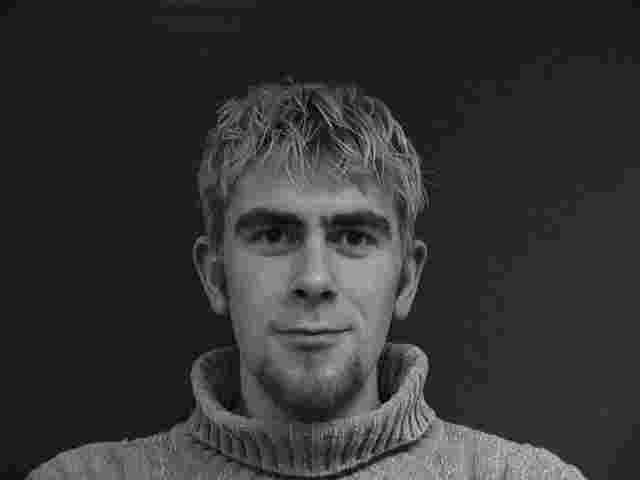
\includegraphics[keepaspectratio=true,
    width=\textwidth]{images/gs0_0.10_quality.jpg}
    \caption{压缩图}
  \end{subfigure}
  \caption{质量因子为10时的压缩操作对gs0.jpg的影响}
\label{fig:quality-ex-img}
\end{figure}

调整上示原图的质量因子$Q \in [0, 1]$、步长为$0.1$(在$[0.9, 1]$之间步长
为$0.01$)后,分别统计与原图的距离,可作如下的散点图
\begin{figure}[H]
  \centering
  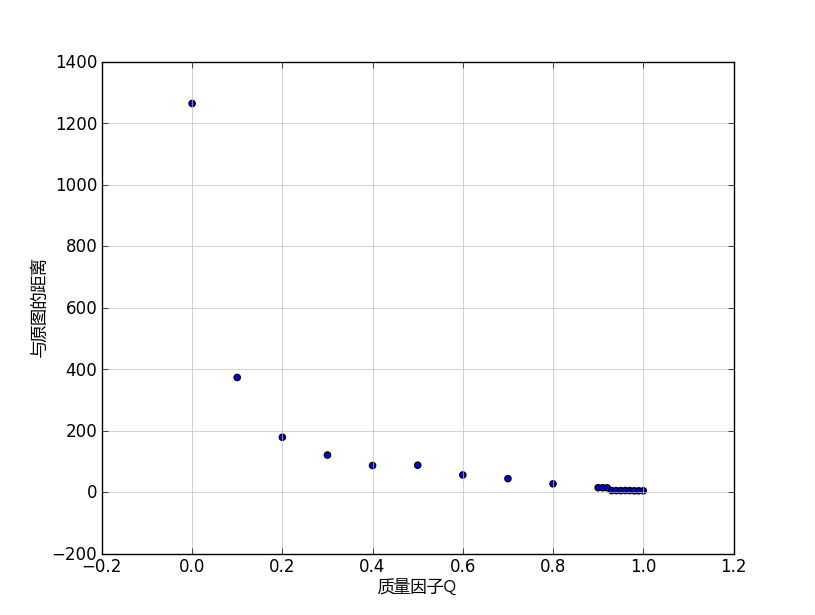
\includegraphics[keepaspectratio=true,
  scale=0.6]{images/quality_gs0.png}
  \caption{对gs0.jpg的压缩操作统计}
  \label{fig:quality-gs0-scatter-plot}
\end{figure}

\begin{figure}[H]
  \centering
  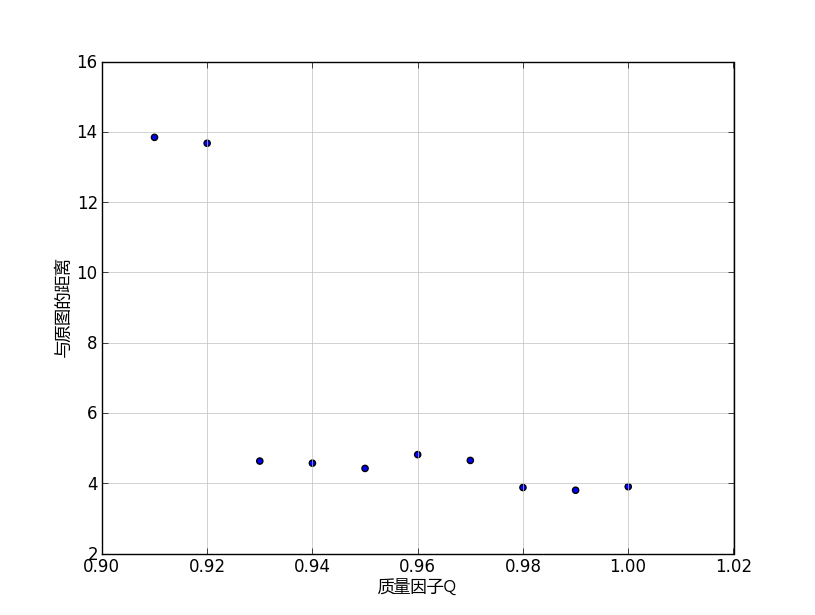
\includegraphics[keepaspectratio=true,
  scale=0.6]{images/quality_gs0_0.9_1.png}
  \caption{对gs0.jpg的压缩操作统计($[0.9, 1]$区间)}
  \label{fig:quality-gs0-sub-scatter-plot}
\end{figure}

为不失一般性,选取37张图片做同样处理,统计出散点图,如图
\begin{figure}[H]
  \centering
  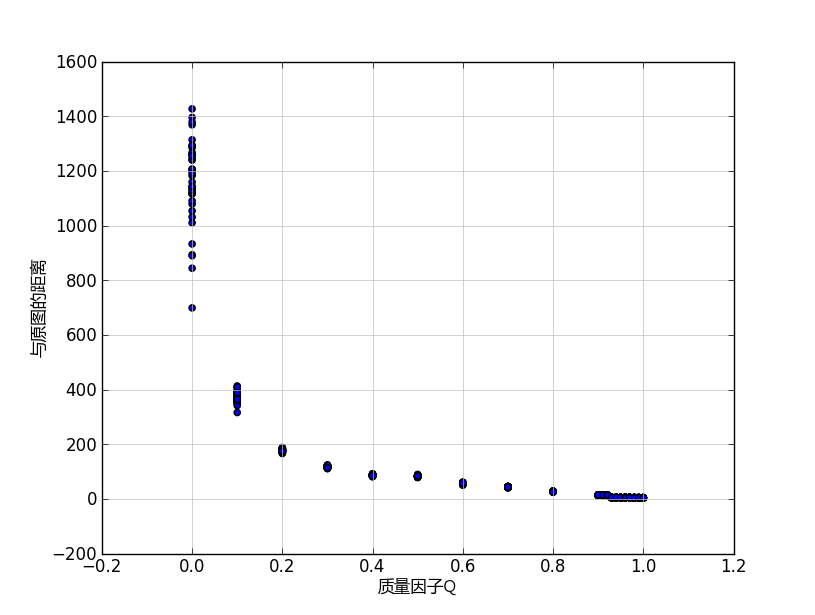
\includegraphics[keepaspectratio=true,
  scale=0.6]{images/quality_all.png}
  \caption{对所有图片的压缩操作统计}
  \label{fig:quality-all-scatter-plot}
\end{figure}

\begin{figure}[H]
  \centering
  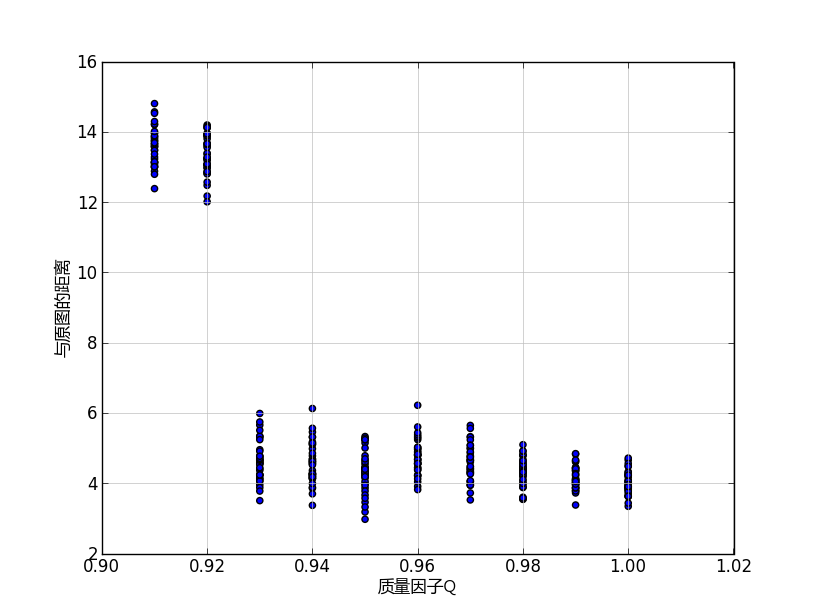
\includegraphics[keepaspectratio=true,
  scale=0.6]{images/quality_all_0.9_1.png}
  \caption{对所有图片的压缩操作统计($[0.9, 1]$区间)}
  \label{fig:quality-gs0-sub-scatter-plot}
\end{figure}

从图中可以看出来,本算法有较好的抗压缩性能,即使图片质量被调整为$10\%$,
与原图的距离仍然小于$500$。




\chapter{总结}
\label{chap:summary}

\section{创新性}
\label{sec:creative-points}

多媒体生物特征数据需要安全存储,同时也要求可以支持内容检索功能。传统加
密处理后的数据一般无法有效进行内容检索,更无法找寻同类或相似的图像或其
它生物特征数据。

基于加密数据库的内容检索,其目标是提供关于加密文档的、高效准确的搜索能
力,并且在搜索时应不需要先解密文档。本系统采用不改变图像特征统计特性的
方法、对特定编码格式的图像文件(JPEG格式)进行特殊的加密处理,算法具有
快速性、简单性、安全性、鲁棒性等性质。

本系统可以实现具有一般权限的操作员在无法获知明文图像的条件下,对多媒体
生物特征数据进行内容检索和管理,能够搜索到相同内容或近似内容的对象数据。
该安全检索系统可以容忍多数的不影响内容的多媒体处理操作,并且其检索性能
不受加密处理影响。

\section{工作综述}
\label{sec:work-overview}

本系统涉及到数学、密码学、图像编码与网络通信等多个学科领域,涵盖了离散
余弦变换、Logistic混沌系统等知识,运用了numpy、opencv等关键技术,针对内
容检索系统的明文内容可能被非法使用等安全问题,设计并实现了一个基于内容
的生物特征图像安全检索系统。

项目团队于2013年2月成立,至今约4个月的时间。在这4个月中,项目成员在大量
课业压力下和指导老师的指导下,进行相关背景知识的调研和学习、系统的设计、
开发与测试,文档的编写与修改。

由于项目成员均是第一次参与到具有较多专业知识系统的开发中、对专业知识的
储备较少,而且课业繁重,项目一度处于停滞状态。但在指导老师的帮助下,项
目成员自发地投身于相关论文的阅读,相关函数库的自学,和程序代码的编制中。
在牺牲了大量的休息娱乐时间之后,较好的完成了设计目标,实现了一个具有良
好图形用户界面的、稳定且快速的系统。

本次项目开发中,项目组成员自学了多种技术手段,并以大量代码的形式,将它
们运用到实践中,锻炼了动手能力,体会到了理论与实践之间不小的差距。在文
档的撰写中也练习了平时很少有机会运用的文档写作技巧及相关软件。

\section{后续工作}
\label{sec:next-step}

由于能力与时间的限制,本系统功能未能做到完善,需要做进一步的调查与研究。
不足主要在以下几方面:
\begin{itemize}
\item 寻求可在保留检索用统计特性的同时,置乱无关统计特性的方法并实现之;
\item 寻找更好的客户端密钥管理方案并实现之;
\item 服务端管理功能不足,增加必要的图像元信息以便对密图集做更细致的管理。
\end{itemize}


\begin{thebibliography}{9}
\bibitem{li2011} 李进, 徐红.
 \emph{基于MD5算法和Logistic映射的图像加密方法研究}[J]. 信息网络安全,
 2011, (8): 25 - 26, 47.
\bibitem{yang2011} 杨恒欢, 冯涛, 荆锐. \emph{一种黑洞数和Logistic混沌序列的图像加密
  应用}[J]. 上海第二工业大学学报, 2011, 28(4): 287.
\bibitem{lu2007} 陆大兴,廖晓峰,韩洁等. \emph{基于Logistic映射与排序变
    换的图像加密算法}
[J].计算机技术与发展,2007,17(12):27-30.
\end{thebibliography}

\end{document}
